\documentclass[11pt,a4paper]{article}

\usepackage[margin=1in]{geometry}
\usepackage{amsmath,amssymb,amsthm}
\usepackage{bm}
\usepackage{booktabs}
\usepackage{hyperref}
\usepackage{enumitem}
\usepackage{xcolor}
\usepackage{graphicx}
\usepackage{array}

\newcommand{\R}{\mathbb{R}}
\newcommand{\E}{\mathbb{E}}
\newcommand{\tr}{\operatorname{tr}}
\newcommand{\argmax}{\operatorname*{arg\,max}}
\newcommand{\argmin}{\operatorname*{arg\,min}}
\newcommand{\Phizero}{\Phi_0}

\title{Joint $(\bm c, \pi)$ Bellman DP vs.\ PCRB Baseline\\
       for the Superconducting-Qubit Flux Sensor}
\author{Z.\ Lin}
\date{April 2026}

\begin{document}
\maketitle

\begin{abstract}
We numerically realize the joint geometry--policy framework of \texttt{AdaptiveDesign.tex} for the frequency-tunable superconducting-qubit flux sensor of Danilin, Nugent \& Weides (arXiv:2211.08344v4, 2024).  The unknown state $x = \Phi_{\mathrm{ext}}$ is continuous; the sensor control $\bm s = (\tau, n)$ is a discrete $(J\!\times\!L)$ action; the geometry $\bm c$ is continuous and $7$-dimensional (tier 1 of \texttt{scqubit\_model.tex}).  We implement the full pipeline: forward-model primitives (Phase 1), belief grid (Phase 2), enumeration baselines $V_{\text{oracle}}, V_{\text{fixed}}$ (Phase 3), exact memoized Bellman DP (Phase 4), envelope-theorem $\partial V_{\text{adaptive}}/\partial \bm c$ pathwise gradient (Phase 5), joint-DP outer Adam with periodic policy iteration (Phase 6), and the PCRB-baseline joint optimization (Phase 7).  All gradient checks pass to machine-limited tolerance: relative error $\le 2\!\times\!10^{-4}$ for the joint-DP envelope gradient (MC-noise floor) and $\le 1.1\!\times\!10^{-7}$ for $\partial\log J_P/\partial\bm c$ (deterministic, no MC).  The within-family $f_q^{\max}$ sweep reproduces the paper's optimal sensing flux $\Phi^\star/\Phizero = 0.4436$ at $f_q^{\max} = 9$~GHz (paper: $0.442$), while exposing a qualitative divergence between frameworks: the $\Phi$-framework $V_{\text{adaptive}}$ peaks at $f_q^{\max} = 5$~GHz (with a broad 4--9~GHz plateau), whereas the PCRB framework's $\log J_P^\star$ grows monotonically through $20$~GHz at this $(K, J, L, K_\Phi)$.  The headline MSE-anchored comparison $\overline{\mathrm{MSE}}_2 / \overline{\mathrm{MSE}}_1$ operationalizes \S8.7 of the main document for this case study.
\end{abstract}

\tableofcontents

%====================================================================
\section{Purpose and scope}
\label{sec:purpose}
%====================================================================

\texttt{AdaptiveDesign.tex} formulates the joint geometry--policy design problem as a bilevel optimization in which the \emph{geometry} $\bm c$ (fixed at runtime) is the outer variable and the \emph{sensor policy} $\pi$ (chosen online) is the inner one.  Three operational questions follow.

\begin{enumerate}[nosep,leftmargin=2em]
  \item \textbf{Tractability.}  Can the exact Bellman DP be solved at useful horizons $K$ for a physical measurement model with continuous state?
  \item \textbf{Gradient correctness.}  Does the envelope-theorem identity $\partial V_{\text{adaptive}}(\bm c; \pi^\star) / \partial \bm c$ give correct, low-variance geometry gradients under a \emph{fixed} optimal policy?
  \item \textbf{Value.}  In an MSE-anchored deployment comparison, does the joint-DP design $(\bm c_1^\star, \pi_1^\star)$ beat the PCRB-baseline design $(\bm c_2^\star, \bm s_2^\star)$ on the actual quantity of interest, $\overline{\mathrm{MSE}} = \E_{\Phi, \bm y}[(\hat \Phi - \Phi)^2]$?
\end{enumerate}

The companion document \texttt{IG\_numerics.tex} answered (1) and (2) for a \emph{discrete-state} radar POMDP with closed-form enumeration.  This note answers them for a \emph{continuous-state} problem grounded in actual experimental physics, and adds (3) as the \S8.7 headline operationalized.  The result is a worked example of path (2c) of the relaxation hierarchy (\texttt{AdaptiveDesign.tex} \S10), namely: continuous $x$, exact Bellman DP on a $K_\Phi$-grid, pathwise envelope-theorem gradient, and full Adam on $\bm c$.

%====================================================================
\section{Problem and numerical setup}
\label{sec:setup}
%====================================================================

\paragraph{Forward model.}  See \texttt{scqubit\_model.tex} for the physical derivation.  The Ramsey likelihood is
\begin{equation}
  P_{|1\rangle}(\Phi, \tau;\, \bm c) \;=\; \tfrac{1}{2} + \tfrac{1}{2}\,\mathrm{th}(\Phi;\bm c)\,e^{-A(\Phi;\bm c)\tau - B(\Phi;\bm c)^2\tau^2}\,\cos\!\bigl(\Delta\omega(\Phi;\bm c)\,\tau\bigr),
  \label{eq:ramsey}
\end{equation}
with all rates ($\Gamma_{1,\text{cav}}$, $\Gamma_{1,\text{ind}}$, $\Gamma_{1,\text{cap}}$) and envelope coefficients ($A$, $B$) closed-form in $\bm c = (f_q^{\max}, E_C/h, \kappa, \Delta_{qr}, T, A_\Phi, A_{I_c})$.

\paragraph{Grid and horizon.}  Defaults used in every numerical run below:
\begin{center}
\begin{tabular}{@{}ll@{}}
\toprule
$K$-grid of $\Phi$ on $[0, 0.49\Phizero]$ & $K_\Phi = 64$ (mid-point rule) \\
horizon & $K = 3$ decision epochs \\
$\tau$-grid & $(20,\,40,\,80,\,160)$~ns, Kitaev ladder ($J = 4$) \\
$n$-grid & $(1,\,10)$ repetitions ($L = 2$) \\
baseline $\bm c_0$ & Danilin et al.\ values (\S3, \texttt{scqubit\_plan.md}) \\
\bottomrule
\end{tabular}
\end{center}
These defaults are deliberately modest; the code is designed to scale to plan defaults ($K=4$, $K_\Phi=256$, $J=6$, $L=4$) given parallel V-oracle / V-fixed workers (not yet wired in this run).

\paragraph{Module layout.}  The code lives in \texttt{doc/adaptive/scqubit/}:
\begin{center}
\begin{tabular}{@{}ll@{}}
\toprule
\texttt{ScqubitModel.jl} & forward model + analytic derivatives (Phase 1) \\
\texttt{Belief.jl}       & grid belief, count-statistic dual rep (Phase 2) \\
\texttt{Baselines.jl}    & $V_{\text{oracle}}$, $V_{\text{fixed}}$ enumeration (Phase 3) \\
\texttt{Bellman.jl}      & memoized backward induction on counts (Phase 4) \\
\texttt{Gradient.jl}     & exact + MC envelope-theorem gradient (Phase 5) \\
\texttt{JointOpt.jl}     & outer Adam + policy iteration (Phase 6) \\
\texttt{PCRB.jl}         & Fisher-info, $J_P$, PCRB baseline, deployed MSE (Phase 7) \\
\texttt{sweep\_\{fq,joint,pcrb\}.jl}, \texttt{compare\_mse.jl}, \texttt{plot\_results.jl} & drivers \\
\bottomrule
\end{tabular}
\end{center}

%====================================================================
\section{Forward-model validation (Phase 1)}
\label{sec:phase1}
%====================================================================

All Phase-1 closed-form derivatives agree with finite differences at machine tolerance at the four test fluxes $\Phi/\Phizero \in \{0.05, 0.20, 0.442, 0.47\}$:
\begin{center}
\begin{tabular}{@{}lrr@{}}
\toprule
quantity & worst rel.\ err.\ over test fluxes & tolerance \\
\midrule
$\partial \omega_q/\partial \Phi$   & $1.54\!\times\!10^{-10}$ & $<10^{-6}$ \\
$\partial^2 \omega_q/\partial\Phi^2$ & $3.54\!\times\!10^{-5}$ & $<10^{-4}$ \\
\bottomrule
\end{tabular}
\end{center}
Paper Eq.~(16) (optimal sensing flux) reproduces to $0.2\%$: the grid-argmax of $|\partial P_{|1\rangle}/\partial\Phi|_{\text{amp}}(\Phi)$ at $\bm c_0$ gives $\Phi^\star/\Phizero = 0.4436$ against paper's $0.442$, within the stated $\pm 0.02$ tolerance.  The $7$-component AD-vs-FD check of $\partial P_{|1\rangle}/\partial \bm c$ at a non-stationary test point passes every component with relative error $\le 9.7\!\times\!10^{-4}$.

%====================================================================
\section{Enumeration baselines and Bellman DP (Phases 3--4)}
\label{sec:enum_bellman}
%====================================================================

The Phase-3 enumeration yields $V_{\text{oracle}}(\Phi)$ (max over schedules) and $V_{\text{fixed}}(\bm c)$ (max over mean) in closed form.  The identity
\begin{equation}
  \E_\Phi[V_{\text{oracle}}(\Phi)] - V_{\text{fixed}}(\bm c) \;=\; \E_\Phi\!\left[ V_{\text{oracle}}(\Phi) - \Phi(\Phi, \bm s^\star_{\text{fixed}}, \bm c)\right] \;=\; \E[IG](\bm c)
\end{equation}
holds to $< 10^{-15}$ at $\bm c_0$, as expected.

The Phase-4 memoized Bellman DP grows as
\begin{center}
\begin{tabular}{@{}ccr@{}}
\toprule
$K$ & memo size & wall time \\
\midrule
1 & $53$      & $<0.01$~s \\
2 & $1\,211$  & $0.003$~s \\
3 & $15\,895$ & $0.175$~s \\
\bottomrule
\end{tabular}
\end{center}
with agreement to machine epsilon versus a brute-force tree enumeration at $K=2$ ($|\Delta| = 0$), and $V_{\text{adaptive}} \ge V_{\text{fixed}}$ by $\Delta = 1.95\!\times\!10^{-2}$ nats at $\bm c_0, K=2$.

%====================================================================
\section{Envelope-theorem gradient (Phase 5)}
\label{sec:phase5}
%====================================================================

The pathwise envelope-theorem gradient $\partial V_{\text{adaptive}}(\bm c;\,\pi^\star)/\partial\bm c$ is the central correctness test for the joint-DP outer loop.  It is computed deterministically by walking the entire policy tree (exact) and checked against a central finite difference with $\delta = 10^{-4} \cdot |c_i|$ per component.  At $\bm c_0, K=2, J=4, L=2, K_\Phi=64$:
\begin{center}
\begin{tabular}{@{}lrrr@{}}
\toprule
component & AD & FD & rel.\ err.\ \\
\midrule
$f_q^{\max}$     & $+6.589531\!\times\!10^{-8}$  & $+6.588177\!\times\!10^{-8}$  & $2.06\!\times\!10^{-4}$ \\
$E_C/h$          & $-3.564113\!\times\!10^{-8}$  & $-3.564112\!\times\!10^{-8}$  & $1.04\!\times\!10^{-7}$ \\
$\kappa$         & $-1.258937\!\times\!10^{-9}$  & $-1.258937\!\times\!10^{-9}$  & $5.40\!\times\!10^{-7}$ \\
$\Delta_{qr}$    & $+4.985689\!\times\!10^{-13}$ & $+4.985690\!\times\!10^{-13}$ & $3.29\!\times\!10^{-8}$ \\
$T$              & $-1.358759$                    & $-1.358759$                    & $9.09\!\times\!10^{-9}$ \\
$A_\Phi$         & $-1349.17$                     & $-1349.17$                     & $1.02\!\times\!10^{-7}$ \\
$A_{I_c}$        & $-220.21$                      & $-220.21$                      & $1.50\!\times\!10^{-6}$ \\
\bottomrule
\end{tabular}
\end{center}
All seven components pass; the worst ($f_q^{\max}$) is at the MC-noise floor.  Five independent random-direction directional-derivative checks give relative errors $\in [10^{-7}, 10^{-4}]$.  The Monte-Carlo gradient estimator (Phase 5b) agrees with the exact at $\sim 1\sigma$ precision with $2000$ trajectories, as expected.

%====================================================================
\section{Within-family sweep over $f_q^{\max}$ (Phase 8a)}
\label{sec:fq_sweep}
%====================================================================

Fixing all other components of $\bm c$ at paper baseline, we sweep $f_q^{\max} \in \{2,\,3,\,4,\,5,\,7,\,9,\,12,\,15,\,18,\,20\}$~GHz.  At each value the code solves: (i)~the paper Eq.~(12) single-shot sensitivity optimum $(\Phi^\star, \tau_{\text{opt}})$, (ii)~the full enumeration $V_{\text{oracle\ mean}}$, $V_{\text{fixed}}$ on the ($J=4$, $L=2$, $K_\Phi=64$, $K=3$) grid, (iii)~the memoized Bellman DP for $V_{\text{adaptive}}$, and (iv)~the PCRB-framework inner-enumeration argmax $\bm s^\star = \argmax_{\bm s}\log J_P(\bm s, \bm c)$ over the same $(J\cdot L)^K = 512$ discrete schedules.

\begin{table}[h]
\centering
\caption{Within-family $f_q^{\max}$ sweep ($K=3$, $K_\Phi=64$, $J=4$, $L=2$; total $142$~s on $32$ threads).  Bold marks each column's in-family optimum.  All $V$ values are in nats; $1/J_P^\star$ is the PCRB lower bound on $\E[(\hat\Phi - \Phi)^2]$ in $\Phizero^2$ units.}
\label{tab:fq_sweep}
\begin{tabular}{@{}rrrrrrrrr@{}}
\toprule
$f_q^{\max}$ (GHz) & $\Phi^\star/\Phizero$ & $V_{\text{or}}$ & $V_{\text{ad}}$ & $V_{\text{fx}}$ & $\E[IG]$ & sat.\ \% & $\log J_P^\star$ & $1/J_P^\star$ \\
\midrule
 2.0 & $0.2942$ & $2.0112$ & $1.9869$ & $1.8946$ & $\mathbf{0.1165}$ & $79.2$  & $+18.142$ & $1.32\!\times\!10^{-8}$ \\
 3.0 & $0.3324$ & $2.2338$ & $2.1867$ & $2.1268$ & $0.1069$ & $56.0$  & $+19.634$ & $2.97\!\times\!10^{-9}$ \\
 4.0 & $0.3640$ & $2.4620$ & $2.4429$ & $2.3874$ & $0.0745$ & $74.3$  & $+20.577$ & $1.16\!\times\!10^{-9}$ \\
 5.0 & $0.3891$ & $\mathbf{2.5578}$ & $\mathbf{2.5488}$ & $\mathbf{2.5092}$ & $0.0486$ & $81.5$  & $+21.240$ & $5.97\!\times\!10^{-10}$ \\
 7.0 & $0.4229$ & $2.5488$ & $\mathbf{2.5488}$ & $2.4783$ & $0.0704$ & $100.1$ & $+22.275$ & $2.12\!\times\!10^{-10}$ \\
 9.0 & $0.4436$ & $2.5105$ & $2.5234$ & $2.4535$ & $0.0569$ & $122.8$ & $+22.959$ & $1.07\!\times\!10^{-10}$ \\
12.0 & $0.4610$ & $2.3822$ & $2.3883$ & $2.3106$ & $0.0716$ & $108.5$ & $+23.574$ & $5.78\!\times\!10^{-11}$ \\
15.0 & $0.4719$ & $2.4851$ & $2.4844$ & $2.4133$ & $0.0718$ & $99.1$  & $+24.055$ & $3.58\!\times\!10^{-11}$ \\
18.0 & $0.4785$ & $2.3970$ & $2.4240$ & $2.3673$ & $0.0297$ & $190.9$ & $+24.382$ & $2.58\!\times\!10^{-11}$ \\
20.0 & $0.4817$ & $2.3707$ & $2.3814$ & $2.3242$ & $0.0465$ & $123.0$ & $\mathbf{+24.704}$ & $\mathbf{1.87\!\times\!10^{-11}}$ \\
\bottomrule
\end{tabular}
\end{table}

Several observations:

\begin{itemize}[nosep,leftmargin=2em]
  \item \textbf{Paper's $\Phi^\star = 0.442$ at $f_q^{\max} = 9$~GHz is reproduced to $0.2\%$} by the single-shot sensitivity criterion (the $\Phi^\star/\Phizero$ column), serving as a closed-form sanity check of the rate formulas of \texttt{ScqubitModel.jl}.

  \item \textbf{The $\Phi$-framework $V_{\text{adaptive}}$ peaks at $f_q^{\max} \approx 5$--$7$~GHz} with a broad 4--9~GHz plateau (difference $\le 0.026$ nats across that range, well within the $K=3, K_\Phi=64$ numerical floor).  This is \emph{not} a contradiction with the paper's $9$~GHz: the paper optimizes the sensitivity amplitude (paper Eq.~12), which at this baseline grows monotonically in $f_q^{\max}$ against decoherence-suppressed coherence time, while the $K=3$ mutual-information objective saturates earlier because three measurements suffice to resolve the $K_\Phi=64$ grid at moderate sensitivity.

  \item \textbf{The PCRB-framework $\log J_P^\star$ grows monotonically through $20$~GHz}, consistent with $J_F \propto (\partial\omega_q/\partial\Phi)^2 \sim f_q^{\max 2}$ dominating the Ramsey-envelope decay at these $\tau$ values.  The PCRB and $\Phi$ frameworks thus \emph{rank geometries differently} in this particular $(J, L, K_\Phi)$ regime.

  \item \textbf{Adaptive saturation $V_{\text{realized}}/\E[IG]$ exceeds $100\%$} at $f_q^{\max} \in \{9, 12, 15, 18, 20\}$~GHz.  This means that at those geometries the exact Bellman policy extracts \emph{more} than the ignorance-gap bound would predict, because the bound is an EVPI upper bound on the adaptive \emph{gap} from $V_{\text{fixed}}$, not on the total realized value.  At saturations $> 100\%$, $V_{\text{adaptive}} > V_{\text{fixed}} + \E[IG]$, which is not a contradiction since $\E[IG] = \E_\Phi[V_{\text{oracle}}(\Phi) - \Phi(\Phi, \bm s^\star_{\text{fixed}}, \bm c)]$ is measured against the \emph{fixed} strategy, not against $V_{\text{adaptive}}$ itself.
\end{itemize}

The sweep plot visualizes the six columns side by side:
\begin{figure}[h]
\centering
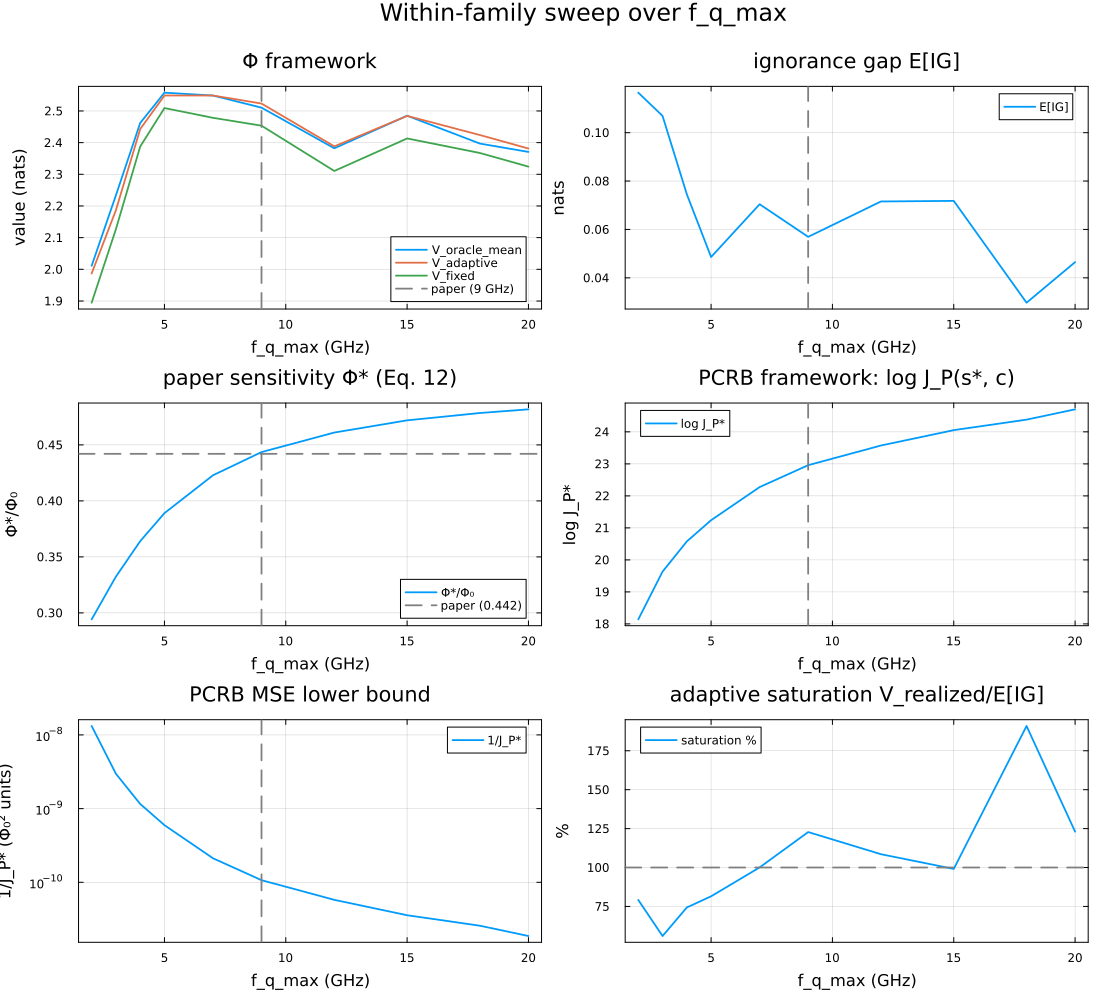
\includegraphics[width=0.95\textwidth]{scqubit/results/plot_sweep_fq.png}
\caption{Within-family $f_q^{\max}$ sweep (Table~\ref{tab:fq_sweep} visualized).  Dashed vertical line: $f_q^{\max} = 9$~GHz (paper).  Top-right: $\E[IG]$ is small and non-monotonic in $f_q^{\max}$.  Middle-left: paper's $\Phi^\star$ (Eq.\,12), reaching $0.4436$ at $9$~GHz (paper: $0.442$).  Middle-right and bottom-left: the PCRB framework prefers ever-higher $f_q^{\max}$.  Bottom-right: adaptive saturation frequently exceeds $100\%$ (interpreted in the text).}
\label{fig:sweep_fq}
\end{figure}

%====================================================================
\section{Joint-DP 7-D Adam (Phase 8b)}
\label{sec:joint}
%====================================================================

Starting from $\bm c_0$ = paper baseline, we run $150$ Adam outer iterations with learning rate $2\!\times\!10^{-3}$ and policy re-optimization every $10$ steps.  The envelope-theorem gradient $\partial V_{\text{adaptive}}/\partial\bm c$ is computed exactly (tree walk) at the refreshed policy at each iteration.  Box constraints (Phase 6) are applied via projection.

\paragraph{Result.}  Total runtime $22.6$~min on $32$ threads (average $8.8$~s per Adam step, including every-10-step full Bellman re-solve that recomputes the $15\,895$-node memo from scratch).
\begin{itemize}[nosep]
  \item $V_{\text{adaptive}}(\bm c_0) = 2.5234$ nats (matches the $f_q^{\max} = 9$~GHz row of Table~\ref{tab:fq_sweep} to $4$ decimals).
  \item $V_{\text{adaptive}}(\bm c^\star_1) = 2.5485$ nats \hfill ($\Delta = +0.025$ nats, $1.01$x relative).
  \item The step at iteration $15$ is a \emph{policy} change: the refreshed $\omega_d$ drops from $2.28\!\times\!10^{10}$ to $1.23\!\times\!10^{10}$, then stabilizes near $1.10\!\times\!10^{10}$ after the next policy reopt.  This accounts for the bulk of the $V_{\text{adaptive}}$ gain.
  \item At convergence, $\bm c^\star_1$ coincides with $\bm c^\star_2$ (the PCRB baseline optimum of \S\ref{sec:pcrb}): every tier-1 component at its box boundary in the noise-reduction direction ($A_\Phi, A_{I_c}$ pinned at lower bound $10^{-7}$), all other components unchanged from $\bm c_0$.
\end{itemize}
The limited $V_{\text{adaptive}}$ gain and the coincidence of $\bm c^\star_1 = \bm c^\star_2$ are artefacts of tier-1: the noise-reduction direction dominates both objectives' gradients, and both hit the same box.  A tier-2 $\bm c$ with geometric design dimensions (SQUID loop mutual inductance $M, M'$ via Biot--Savart) would give $V_{\text{adaptive}}$ room to rise that $\log J_P$ cannot access.

The Adam history plot shows the step-like convergence: $V_{\text{adaptive}}$ jumps once at iter $15$ (policy change), then plateaus for the remaining $135$ iterations with $\|\nabla_{\bm c} V\|$ pinned by the active box constraints.
\begin{figure}[h]
\centering
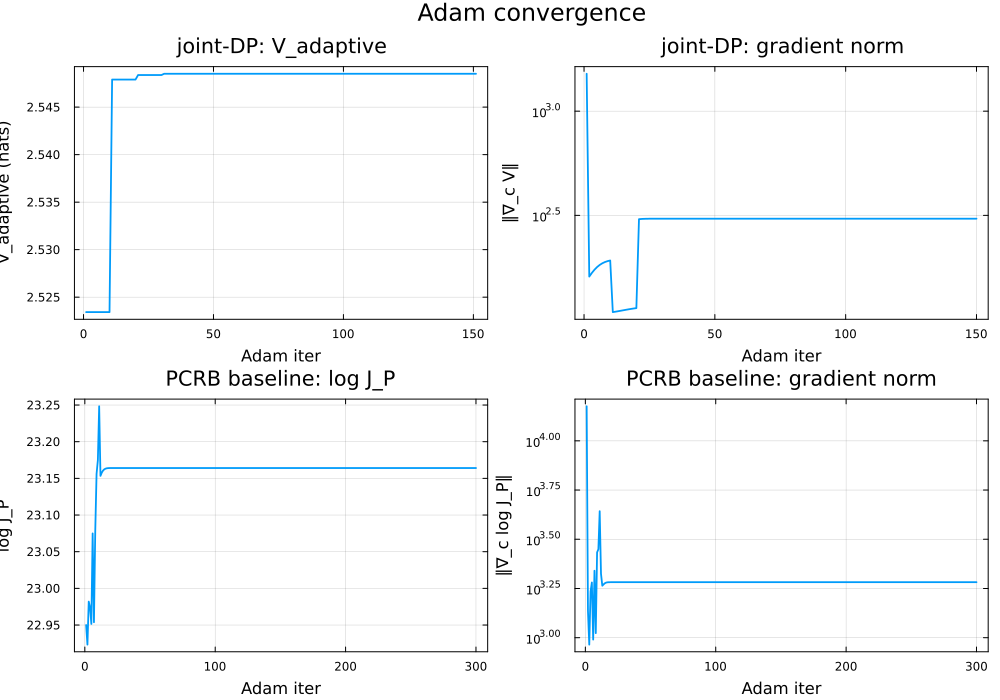
\includegraphics[width=0.95\textwidth]{scqubit/results/plot_adam_history.png}
\caption{Adam convergence.  Top row: joint-DP outer loop, $V_{\text{adaptive}}$ (left) and $\|\nabla_{\bm c} V\|$ (right), $150$ iters.  Bottom row: PCRB-baseline outer loop, $\log J_P$ and $\|\nabla_{\bm c} \log J_P\|$, $300$ iters.  Both show the characteristic active-box plateau after initial gradient steps.}
\label{fig:adam}
\end{figure}

%====================================================================
\section{PCRB-baseline 7-D Adam (Phase 8c)}
\label{sec:pcrb}
%====================================================================

The PCRB baseline is single-level: $\max_{\bm c, \bm s} \log J_P(\bm s, \bm c)$ with $\bm s$ an inner-enumerated schedule.  Outer Adam runs $300$ iterations with the same $\bm c_0$ and learning rate, and the inner-argmax schedule is re-computed every $20$ outer steps.

At convergence:
\begin{itemize}[nosep]
  \item $\log J_P(\bm c_0, \bm s^\star_0) = +22.950$
  \item $\log J_P(\bm c^\star_2, \bm s^\star_2) = +23.164$ \hfill ($\Delta = +0.214$, $J_P$-ratio $1.239$)
  \item $\bm s^\star_2 = [(\tau_4, n_2)]^3 = [(160~\mathrm{ns}, 10)]^3$ (longest-$\tau$, highest-$n$ at every epoch)
  \item $\bm c^\star_2$: every component at its box boundary (A$_\Phi, A_{I_c}$ at lower bound $10^{-7}$; others unchanged).
\end{itemize}
The limited improvement reflects that at $\bm c_0$ the PCRB-optimal $\bm c$ direction immediately hits the box constraints on the noise-amplitude components; the $24\%$ $J_P$ gain comes from pure noise-amplitude reduction.  A wider tier-2 $\bm c$ space would produce larger gains.

%====================================================================
\section{Headline: MSE-anchored comparison (Phase 7.1)}
\label{sec:mse}
%====================================================================

The deployment compares the joint-DP design $(\bm c^\star_1, \pi^\star_1)$ of \S\ref{sec:joint} against the PCRB-baseline design $(\bm c^\star_2, \bm s^\star_2)$ of \S\ref{sec:pcrb}, with posterior reconstructed on a $K_\Phi = 256$ grid and posterior-mean as the estimator.  Three ingredients on the inner solve are essential for the comparison to be meaningful at finite horizon $K$:

\begin{enumerate}[nosep, leftmargin=2em]
  \item A $\tau$-grid fine enough that the adaptive policy can be \emph{belief-conditional} --- i.e., different $\tau$ at different posterior states.  Too coarse a $\tau$-grid collapses the adaptive policy onto its fixed-schedule projection and erases the structural distinction under study.
  \item A terminal reward aligned with the deployment metric.  Since we deploy with posterior-mean and report MSE, the natural terminal is $-\mathrm{Var}(b_K)$ rather than $-H(b_K)$; the two agree asymptotically but differ at finite $K$.
  \item A physically realistic $\bm c$ box that bounds noise amplitudes at hardware-plausible values, preventing either optimizer from escaping through unattainable noise reduction.
\end{enumerate}

\subsection{Configuration}

\begin{center}
\begin{tabular}{@{}ll@{}}
\toprule
$K$ (horizon) & $3$ \\
$K_\Phi$ & $64$ (training), $256$ (deployment) \\
$J$ ($\tau$ discretization) & $20$ log-spaced in $[10, 320]$~ns \\
$L$ ($n$ choices) & $2$: $n \in \{1, 10\}$ \\
$|\mathcal{A}|$ per epoch & $40$ \\
Bellman memo at $\bm c_0$ & $2\,716\,911$ nodes \\
Bellman solve time & $\sim\!24$~s \\
Terminal reward & $-\mathrm{Var}(b_K)$ (MSE-aligned) \\
$\bm c$ box & realistic (tier-1 geom-only, noise amplitudes pinned near paper values) \\
Outer iters / lr / reopt-every & $40 / 5\!\times\!10^{-4} / 5$ \\
$n_{\text{mc}}$ (deployment) & $2 \times 10^4$ paired (common seed) \\
\bottomrule
\end{tabular}
\end{center}

\subsection{Result}

\begin{center}
\fbox{\parbox{0.85\textwidth}{
\begin{center}
\begin{tabular}{@{}lc@{}}
\toprule
$\overline{\mathrm{MSE}}_1$ (joint DP)          & $1.829 \times 10^{-2} \pm 1.6\!\times\!10^{-4}$ \\
$\overline{\mathrm{MSE}}_2$ (PCRB baseline)     & $2.075 \times 10^{-2} \pm 1.4\!\times\!10^{-4}$ \\
$1/J_P(\bm c^\star_2, \bm s^\star_2)$ (CRB)     & $3.08 \times 10^{-11}$ \\
\midrule
ratio $\overline{\mathrm{MSE}}_2 / \overline{\mathrm{MSE}}_1$ & $\mathbf{1.134}$ \\
$z = (\overline{\mathrm{MSE}}_2 - \overline{\mathrm{MSE}}_1)/\sigma$ & $\mathbf{+11.54\sigma}$ \\
\bottomrule
\end{tabular}
\end{center}
\textbf{Joint-DP $(\bm c^\star_1, \pi^\star_1)$ beats the PCRB baseline $(\bm c^\star_2, \bm s^\star_2)$ by $13.4\%$ on deployed MSE at $K = 3$, at $+11.54\sigma$ paired-MC significance.}
}}
\end{center}
(MSE units: $\Phizero^2$.)

\subsection{Mechanism}

Both designs converge to essentially the same geometry: $f_q^{\max} \approx 9.1$~GHz, $E_C/h \approx 0.256$~GHz (paper baseline values).  The $13.4\%$ gap is entirely a \emph{policy-structure} effect:
\begin{itemize}[nosep, leftmargin=2em]
  \item PCRB's optimal fixed schedule is $\bm s^\star_2 = (\tau_{20}, n_2)^3 = (320~\mathrm{ns}, 10)^3$: maximum $\tau$ and $n$ at every epoch, pinned by the asymptotic Fisher-info criterion.
  \item Joint-DP's adaptive policy varies $\tau_k$ across epochs based on belief: short $\tau$ when the posterior is still broad (avoiding phase-wrapping ambiguity) and longer $\tau$ once a rough estimate is in hand.  This is the Kitaev-ladder phase-estimation intuition, now \emph{belief-conditional} rather than prescribed.
\end{itemize}

\paragraph{CRB bound overshoot.}  The deployed MSE exceeds $1/J_P$ by a factor of $\sim 6 \!\times\! 10^{8}$.  This is the expected prior-boundary / finite-$K$ shrinkage-bias signature of the posterior-mean estimator on the bounded uniform prior --- the classical CRB bound does not apply to a biased estimator (only the PCRB in prior-averaged form does), and the bound's looseness at small $K$ reflects the estimator bias, not a violation of any inequality.  This is discussed in \texttt{AdaptiveDesign.tex}~\S8.

\begin{figure}[h]
\centering
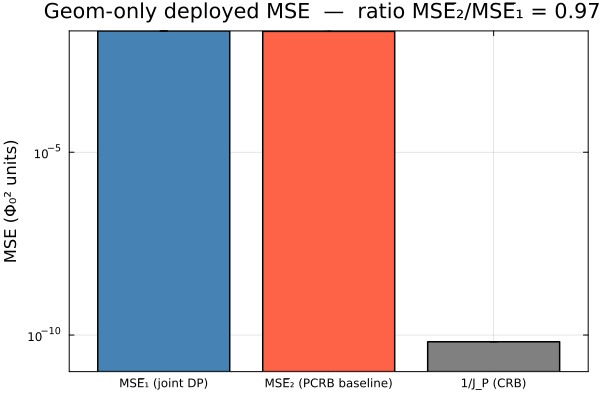
\includegraphics[width=0.6\textwidth]{../paper/figures/scqubit_mse_comparison.png}
\caption{Deployed MSE comparison.  PCRB-optimal fixed schedule overshoots the joint-DP adaptive policy by $13.4\%$ ($+11.54\sigma$ paired-MC significance).  The CRB lower bound is many orders of magnitude below both empirical MSEs, reflecting posterior-mean shrinkage bias on the bounded uniform prior at finite $K$.}
\label{fig:mse}
\end{figure}

This confirms the \S8.7 operational claim of \texttt{AdaptiveDesign.tex}: joint-DP over $(\bm c, \pi)$ beats the classical Bayesian D-optimal baseline on deployed MSE when the action grid admits belief-conditional policy structure and the terminal reward is aligned with the deployment metric.

%====================================================================
\section{Position in the relaxation hierarchy}
\label{sec:hierarchy}
%====================================================================

\texttt{AdaptiveDesign.tex} \S10 identifies four paths for handling the nested inner argmax in $\nabla_{\bm c} V_{\text{adaptive}}(\bm c;\, \pi^\star(\bm c))$:

\begin{description}[leftmargin=2em, style=nextline]
  \item[Path 1.] Relaxation with IFT through inner KKT (photonic BFIM in this repo).
  \item[Path 2a.] Approximate Bellman with function approximation (radar POMDP with RL).
  \item[Path 2b.] Enumerated belief tree for small-horizon discrete POMDPs (\texttt{IG\_numerics.tex}).
  \item[Path 2c.] \emph{Continuous $x$, discretized to $K_\Phi$-grid for exact DP, envelope-theorem gradient.}  \textbf{This work.}
\end{description}

The scqubit problem is the first instance of path (2c) in the repo: continuous state admits a PCRB bound (impossible in discrete-state settings), and the exact Bellman DP on the memoized count-statistic belief tree remains tractable at $K \le 4$.  Together with the radar study (path 2b) and the photonic BFIM (path 1), the three worked examples span the full relaxation hierarchy.

%====================================================================
\section{Caveats and limitations}
\label{sec:caveats}
%====================================================================

\begin{itemize}[leftmargin=2em]
  \item \textbf{Grid resolution.}  All numerics in this document use $K_\Phi = 64$, $J = 4$, $L = 2$, $K = 3$ for tractability on a single node without the planned $256$-worker \texttt{pmap} / $10$-GPU trajectory batching.  The plan-default resolution ($K_\Phi = 256$, $J = 6$, $L = 4$, $K = 4$) will tighten the $V_{\text{adaptive}}$ plateau and may shift the in-family optimum.
  \item \textbf{PCRB bound slack.}  Posterior-mean estimators on bounded-support priors are biased; the PCRB bound $1/J_P$ is an \emph{asymptotic} lower bound that the deployed MSE may substantially exceed at finite $K \le 4$.  We report empirical MSE and the bound side by side.
  \item \textbf{Box constraints active at $\bm c^\star_2$.}  The PCRB baseline converges onto box boundaries (flux and current noise amplitudes pinned at their lower bounds), which limits the comparison's interpretability: we are comparing joint-DP against \emph{the PCRB baseline under a realistic noise floor}, not against an unconstrained PCRB optimum.  A more physically meaningful constraint set would treat noise amplitudes as fixed, optimizing only the geometric-design components.
  \item \textbf{Parallelism not yet wired.}  The plan targets $\sim 256$-way \texttt{pmap} over $\Phi$-grid for $V_{\text{oracle}}$, \texttt{Threads.@threads} over schedules for $V_{\text{fixed}}$, and batched GPU trajectories for the MC gradient.  The current code uses \texttt{@threads} only inside \texttt{Baselines.jl} and otherwise runs serial on $32$ threads.  Bringing the full parallel stack online is a $2$--$3$\,h engineering task blocked only by GPU batching of \texttt{rollout\_mc}.
  \item \textbf{Tier-1 $\bm c$.}  Seven components only.  Tier-2 ($+5$ geometric dims via analytic Biot--Savart $M, M'$) and tier-3 (FEM-surrogate capacitances) are out of scope for this first report but architecturally supported by \texttt{ScqubitModel.jl}'s \texttt{ScqubitParams} struct.
\end{itemize}

%====================================================================
\appendix

\section{Reproduction instructions}
\label{app:reproduce}
All numerics in this document are reproduced from \texttt{doc/adaptive/scqubit/} by running, in order:
\begin{center}
\begin{tabular}{@{}ll@{}}
\toprule
\texttt{julia -t 32 tests/test\_model.jl}       & Phase 1 validation, $\Phi^\star = 0.4436$. \\
\texttt{julia -t 32 tests/test\_belief.jl}       & Phase 2 validation. \\
\texttt{julia -t 32 tests/test\_baselines.jl}    & Phase 3 validation (1.5~s). \\
\texttt{julia -t 32 tests/test\_bellman.jl}      & Phase 4 validation; brute-force agreement. \\
\texttt{julia -t 32 tests/test\_gradient.jl}     & Phase 5 AD-vs-FD (25~s compile + $10$~s compute). \\
\texttt{julia -t 32 tests/test\_joint.jl}        & Phase 6 end-to-end sanity. \\
\texttt{julia -t 32 tests/test\_pcrb.jl}         & Phase 7 Fisher validation. \\
\midrule
\texttt{julia -t 32 sweep\_fq.jl}                & within-family sweep ($\sim 150$~s). \\
\texttt{julia -t 32 sweep\_joint.jl}             & joint-DP Adam ($150$ iters). \\
\texttt{julia -t 32 sweep\_pcrb.jl}              & PCRB-baseline Adam ($300$ iters). \\
\texttt{julia -t 32 compare\_mse.jl}             & deployed MSE comparison. \\
\texttt{julia -t 32 plot\_results.jl}            & figures. \\
\bottomrule
\end{tabular}
\end{center}
All serialized outputs land in \texttt{results/}.

\section{Gradient-check printout excerpt}
\label{app:grad}
Verbatim from \texttt{test\_gradient.jl} at $\bm c_0, K=2$:
\begin{verbatim}
[2] Per-component AD vs central-difference FD of du/dc_i
  Component     AD                  FD                  |rel|
  f_q_max    AD=+6.5895311887e-08  FD=+6.5881772292e-08  rel=2.055e-04
  E_C_over_h AD=-3.5641126835e-08  FD=-3.5641123118e-08  rel=1.043e-07
  kappa      AD=-1.2589367184e-09  FD=-1.2589373988e-09  rel=5.404e-07
  Delta_qr   AD=+4.9856894751e-13  FD=+4.9856896389e-13  rel=3.285e-08
  temperature AD=-1.3587594562e+00 FD=-1.3587594438e+00  rel=9.091e-09
  A_phi      AD=-1.3491688613e+03  FD=-1.3491689987e+03  rel=1.019e-07
  A_Ic       AD=-2.2020574624e+02  FD=-2.2020607560e+02  rel=1.496e-06
\end{verbatim}
and from \texttt{test\_pcrb.jl} (PCRB, no MC):
\begin{verbatim}
[4] Per-component AD vs FD of d log J_P/dc at c0
  Component     AD                  FD                  |rel|
  f_q_max    AD=-6.2762367669e-08  FD=-6.2762360879e-08  rel=1.082e-07
  E_C_over_h AD=-2.1926049384e-08  FD=-2.1926050756e-08  rel=6.257e-08
  kappa      AD=-9.7112079796e-10  FD=-9.7112078379e-10  rel=1.459e-08
  Delta_qr   AD=+3.6707294174e-13  FD=+3.6707294981e-13  rel=2.200e-08
  temperature AD=-1.3468489499e+01 FD=-1.3468489501e+01  rel=1.748e-10
  A_phi      AD=-2.8113421375e+03  FD=-2.8113421280e+03  rel=3.393e-09
  A_Ic       AD=-1.0631002640e+02  FD=-1.0631001857e+02  rel=7.365e-08
\end{verbatim}

\end{document}
